\documentclass[11pt, oneside]{article}   	% use "amsart" instead of "article" for AMSLaTeX format
\usepackage{geometry}                		% See geometry.pdf to learn the layout options. There are lots.
\usepackage{textcomp}
\usepackage{hyperref}  % TODO: see page 94 of latex book
\geometry{letterpaper}                   		% ... or a4paper or a5paper or ... 
%\usepackage[parfill]{parskip}    		% Activate to begin paragraphs with an empty line rather than an indent
\usepackage{graphicx}				% Use pdf, png, jpg, or eps§ with pdflatex; use eps in DVI mode
								% TeX will automatically convert eps --> pdf in pdflatex		
\usepackage{amssymb}

\title{CSCI E-181 Spring 2014 Practical 1}
\author{David Wihl\\
     \texttt{davidwihl@gmail.com}}
%\date{}							% Activate to display a given date or no date

\begin{document}
\maketitle
\section*{Warm-Up}

%\subsection*{Basic K-Means}

\par As a warmup, I synthesized five clusters of data.  I then used a K-Means implementation in Octave I had written for a previous course.\footnote{Machine Learning, Coursera, Prof. Andrew Ng, Completed Jan 2014, \url{https://class.coursera.org/ml-004}} While this implementation was sufficient for the prior course's provided dataset, when I tested it with the synthesized data set, K=5 and random initial centroids, one of the centroids would frequently not converge on any points.

\begin{figure}[h!] 
\centering
\includegraphics[scale=0.6]{randominitialClusters}
\caption{Random Initial Centroids After 1 Iteration}
\end{figure}

I subsequently modified the code to use K-Medoids, choosing one of the sample data points at random as an initial centroid. This worked much better.

\begin{figure}[h!]
\centering
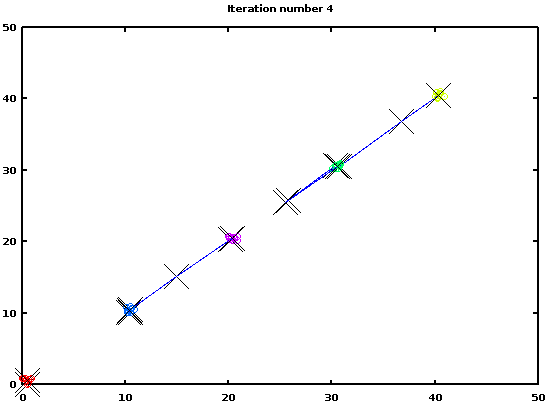
\includegraphics[scale=0.6]{K-Medoid}
\caption{K-Medoids Converge After 4 Iterations}
\end{figure}

\subsection*{CIFAR-10 Image Data}

I then attempted using K-Medoids with the CIFAR-10 Image Data, using the Matlab version of the data with Octave. The training data consists of a 10000x3072 matrix of UInt8. Each row is a 32x32x3 (total 3072 columns) color image, consisting of 1024 red, 1024 green and 1024 blue elements. There are 10 classes in the set (``airplane'', ``automobile'', etc.), so setting K=10 was a rational first step.

Percentage Distribution of K values after normalization and 10 iterations

06
05
04
26
14
13
05
04
03
15

TODO: fill this in
\clearpage

\section*{Recommender System}

For the main part of the exercise, I investigated a series of increasing complex algorithms. 

\subsection*{Pearson Distance}

The first was using Pearson distance from \emph{Programming Collective Intelligence}.\footnote{Programming Collective Intelligence by Toby Segaran. \textsuperscript{\textcopyright} 2007 Toby Segaran, 978-0-596-52932-1.}

\begin{figure}[h!]
\centering
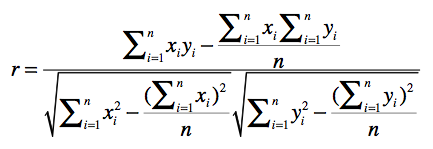
\includegraphics[scale=0.6]{pearson}
\caption{Pearson Correlation Coefficient Approximation}
\end{figure}

Unfortunately Pearson distance is not very effective with sparse data. Given that the training consisted of only 200000 ratings for 131378 books x 12787 users, the ratings were sparse, so Pearson was not very effective at all.

\subsection*{Collaborative Filtering with Regularized Gradient}

\par In the previous Coursera course, I had to build a similar recommender system for movies. (The vectorized Octave implementation can be found in \texttt{cofiCostFunc.m}.) However that data was significantly differently with 1682 movies and 943 critics. The biggest difference was again the sparseness of this problem's data in comparison.

An additional complexity was translating the existing Octave code to Python. While I had significant Python programming experience, I was less familiar with the \texttt{numpy} and \texttt{scipy} vector libraries. The Coursera / Ng class neatly packages the implementation so there were only a few lines of vectorized Octave to add. To reimplement in Python was rapidly taking significantly more code (like 20x!) to get equivalent functionality. 

While I could have adapted the prior Octave code to this problem, I decided not to as 1) I would not have learned as much, 2) I was skeptical that the algorithm would adapt well to the sparseness of the current data set. In my real world experience, data is more sparse and more noisy so it would be more interesting to tackle a new approach.

\subsection*{A More Systematic Approach}

Given the limit of four Kaggle submissions per day, I could not simply attempt a wide variety of different methods. While Kaggle would provide an overall score quality, it did provide enough fine-grained feedback as to which cases were lowering the score. Also, each execution was taking up to 20 minutes on my laptop. So I chose a more systematic approach. First, I created a very simple set of training data. This synthetic training data allowed me to exercise a variety of different permutations and edge cases.

Normal cases:
\begin{itemize}
  \item two very similar users
  \item two very similar books
  \item two or more mostly similar users
\end{itemize}

Pathological cases:
\begin{itemize}
  \item an outlier user (e.g. single review)
  \item a book without any reviews
  \item a user without any reviews
\end{itemize}

This is more of a Test-Driven Development approach where most cases, both plausible and implausible, are defined prior to implementation. \emph{The most limiting factor in this exercise is the number of Kaggle submissions, not the data or the algorithms.} I needed a means to improve the quality of the implementation quickly without using up a Kaggle submission unnecessarily. 

To further improve the quality, I split the 200000 rows of training data into an 80/20 mixture of training and validation data. The validation set enabled me to check that the code would apply readily to the problem data as well verify the accuracy of the predictions. It also enabled me to find which patterns of data had the most error. Different algorithms could be applied depending on the pattern, a kind of simplified ensemble system.

\subsection*{Cosine Distance}

The next algorithm I attempted with a rather simple Cosine Distance \footnote{Guide to Data Mining, Chapter 2 http://guidetodatamining.com/chapter-2/}
calculation.
\begin{figure}[h!]
\centering
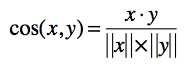
\includegraphics[scale=0.8]{cosine}
\caption{Cosine Distance}
\end{figure}

Since Cosine distance works well with sparse data, it significantly improved the results. This also exercised the synthetic data and testing environment. However I was still below the per-user mean, so the implementation had to increase in sophistication.

\subsection*{Researching the Netflix Solutions}

I read and review the winning Netflix solutions, specifically, Feature-Weighted Linear Stacking \footnote{Sill, et al. http://arxiv.org/pdf/0911.0460.pdf} and Matrix Factorization Techniques \footnote{Volinsky et al. http://www2.research.att.com/~volinsky/papers/ieeecomputer.pdf}. However, as a solo Extension school student without prior \texttt{numpy} experience, I felt I did not have sufficient time to build a reliable implementation of these more sophisticated algorithms. 

\section*{Conclusion}

I really enjoyed this exercise. The Kaggle competition was a strong motivating factor to improve my results, especially as the leaderboard varied day by day or hour by hour. The real world sparse and noisy data, was a more effective learning exercise than the packaged Octave example in my prior Coursera Machine Learning class. The need to use a systematic approach with both clean and pathological test data will be useful both in future exercises for this class as well as real world application.

As an Extension student, I would have liked to have the opportunity to partner with either other Extension students or in-class students. I think this would have improved the learning rate for both me and my potential collaborators. In the Coursera class, I often learned as much as from other students as from the lectures and class material. Of course, I also reciprocated with my practical experience in Machine Learning applications from my day job. Education is blending with a mix of in-class and on-line learning. Like the Kaggle competition, mixing the two would be a more modern, more effective approach. Ensemble learning for the classroom!


\end{document}  
